\section{Der SMD-Assistent im GDS-System}
Die \ac{SMD} enthalten alle wichtigen Informationen um die Strucktur einer Klasse zu beschreiben. Diese Klasseninformationen sollen sp\"ater von einem SMD-Assistent verwaltet werden.

In einer MySQL-Datenbank k\"onnen alle Klasseninformationen abgelegt werden. Zu diesen Informationen z\"ahlen zum Beispiel der Klassenname, Attribute mit Modifier, Methoden mit Modifier Parametern und R\"uckgabetyp. 

Da es sich bei den \ac{SMD} um reine Metadaten handelt, werden keine Methodenr\"umpfe in die \ac{SMD}-Datenbank aufgenommen.

Der Nutzer des \ac{GDS}-Systems gibt \"uber den \ac{UDDE}, also das User Interface, seine Klassen und \ac{AMD} in das System.
Unter \ac{AMD} werden die zu seinen Klassen passenden Instanzen bezeichnet, welche der User der Anwendung zum Speichern \"ubergibt.
Des weiteren legt der \ac{UDDE} die generierten "`strukturellen Metadaten"' in einer Datenbank ab, welche sp\"ater vom SMD-Assistent ausgelesen werden k\"onnen.

Der SMD-Assistent ist also f\"ur das Umwandeln von Klassen in \ac{SMD}s verantwortlich. Nach dem erstellen der \ac{SMD}s werden diese zur Aufbewahrung vom Assistenten dem \ac{GDS} \"ubergeben, welcher die Ablage der Daten in einer Datenbank verwaltet.

Die \ac{SMD}s werden von der Anwendung an verschiedenen Stellen ben\"otigt. Der \ac{CG} wandelt die \ac{SMD}s wieder in Java-Klassen, welche OPM-Konform erzeugt werden. Bei den erstellten Klassen handelt es sich nat\"urlich nur um einfache Ger\"uste, aber mehr wird f\"ur eine Serialisierung beziehungsweise Deserialisierung nicht ben\"otigt.
Die generierten Datenstr\"ome k\"onnwn dann ebenfalls vom \ac{GDS} in einer Datenbank gespeichert werden.

Der \ac{IG} erstellt aus den vom SMD-Assistenten gelieferten \ac{SMD}s Schemen f\"ur JSON und XML. Eine Funktion zur Erstellung des JSON-Schemas aus einer Klasse wird in Kapitel \ref{JSON-Schema} beschreiben.
Auch das entsprechnde Klassenschema soll vom \ac{GDS} in einer Datenbank abgelegt werden.

Der beschriebene Zusammenhang der Komponenten des \ac{GDS} ist im Bild unten noch einmal verdeutlicht.

\begin{figure}[!ht]
\centering
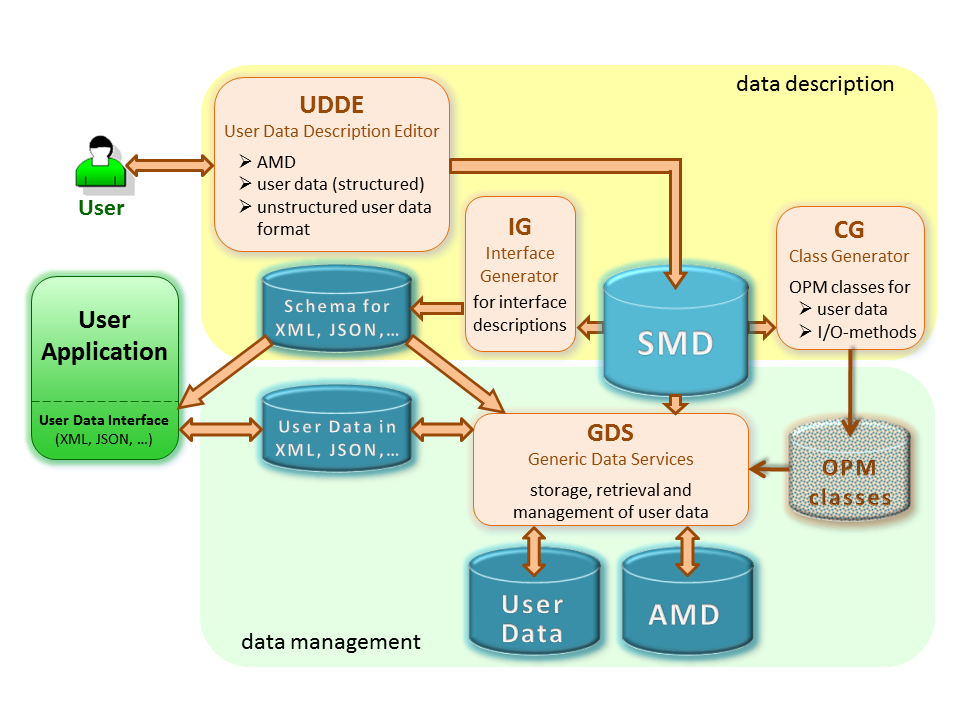
\includegraphics[width=13.5cm]{Bilder/UebersichtGDS}
\title{GDS \"Ubersicht}
\caption{GDS \"Ubersicht}
\centering
\end{figure}

\FloatBarrier

\subsection{Spezifikation des SMD-Assistent}
Im Verlauf der Arbeit wurde zunehmend klar, das die Spezifikation des SMD-Assistent n\"otig wird. Da er, wie im Schaubild oben zu erkennen, zentraler Bestandteil des Projektes ist.
Der SMD-Assistent wurde im Projekt \"offter diskutiert und soll an dieser stelle einmal genauer erleutert werden.

\subsubsection{Funktionen des SMD-Assistent}
Der SMD-Assistent soll die "`strukturellen Metadaten"' aus der Datenbank laden und diese an das \ac{GDS}, den \ac{IG} oder den \ac{CG} weiterreichen. 

Zu einer ObjectID, einer InstanzID oder einem Klassennamen m\"ussen die passenden Metadaten aus der Datenbank geladen werden.
Die geladenen Daten werden in einer Instanz der Klasse \texttt{ClassDecr} zusammengafasst und mittels dieser Instanz \"ubergeben.

Eine Instanz der Klasse \texttt{ClassDecr} enth\"alt mittels der Klassen \texttt{MethodDescr} und \texttt{AttrDecr} alle n\"otigen Informationen um eine Klasse rekonstruieren zu k\"onnen.

\texttt{MethodDescr} enth\"alt eine Methode der Klasse, mit einer Liste von allen Parametern und deren Typen.
Die Klasse \texttt{AttrDecr} hingegen h\"alt jeweils ein Attribut mit dessen Informationen wie zum Beispiel Type und Modifier. \cite{Zil14}

Der Zusammenhang ist im Klassendiagramm der SMD-Klassen noch einmal dargestellt. Im Bild ist aus Gr\"unden der \"Ubersichtlichkeit nicht der gesamte OPM-Klassenbaum abgebildet, sondern lediglich die f\"ur den SMD-Assistent wichtige Klassen sind aufgef\"uhrt.

Einmal aus der Datenbank geladene \ac{SMD}s soll der SMD-Assistent zwischenspeichern, um beim erneuten Abfragen schneller reagieren zu k\"onnen. 

Damit es nicht zu einem Arbeitsspeicher \"uberlauf kommt, muss der SMD-Assistent genau wie alle anderen Assistenten auch eine M\"oglichkeit besitzen den Zwischenspeicher zu verkleinern. Dies soll \"uber einen m\"oglichst effizienten Scheduling-Algorithmus geschehen, welcher Implementiert und auf Effizienz gepr\"uft werden muss.

Hier kommt ein weiterer Assistent zum Einsatz, und zwar der Speicher-Assistent, welcher bei geringem Arbeitsspeicher einen Befehl an alle Assistenten schickt, damit diese ihren Speicherbedarf reduzieren.

\begin{figure}[!ht]
\centering
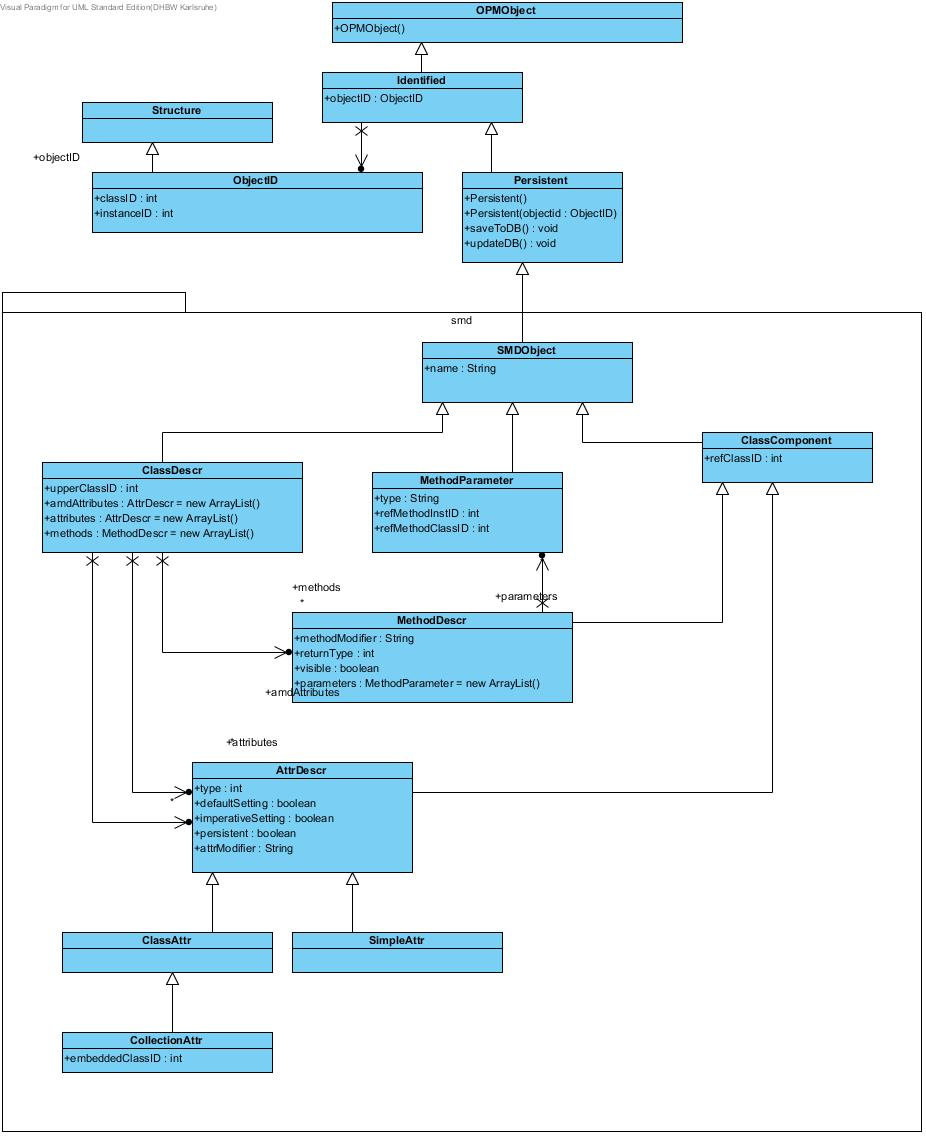
\includegraphics[width=13cm]{Bilder/SMD_Klassen}
\title{Klassendiagramm der SMD-Klassen}
\caption{Klassendiagramm der SMD-Klassen}
\centering
\end{figure}

\subsubsection{Der SMD-Assistent unter Java}
Unter Java kann die Arbeitsweise des SMD-Assistent deutlich vereinfacht werden, da hier die \ac{SMD}s nur bei explizitem verlangen geliefert werden m\"ussen, denn Java verwendet mit den \textit{.class}-Files eigene Metadaten \"uber die eine Verarbeitung unter Java einfacher Umgesetzt werden kann. 
Der SMD-Assistent sollte unter Java also in der Lage sein direkt \textit{.class}-Files zu liefern.